\documentclass[a4paper,11pt]{article}
\usepackage[T1]{fontenc}
\usepackage[utf8]{inputenc}
\usepackage{lmodern}
\usepackage{hyperref}
\usepackage{graphicx}

\title{Project Requirements}
\author{Balz Aschwanden, Raoul Grossenbacher, Florian Jörg}

\begin{document}

\maketitle
%\tableofcontents
\section*{Project Name: StudiHome}

\textbf{Team:} 6 \\
\textbf{Costumer:} Bledar Aga \\

\subsection*{Revision History}
\begin{tabular}{|p{1.2cm}|p{3cm}|p{8cm}|} \hline
  Version & Date & Revision Description \\ \hline
  0.01 & October 8. 2014 &
  \begin{itemize}
  	\item Added use cases and diagram
  	\item Changed user called \textit{student} to \textit{tenant}
  	\item Changed functional requirements for advertisements
  \end{itemize} \\ \hline
  0.02 & October 26. 2014 & 
  \begin{itemize}
  	\item Added minimal information requirement to use case \textit{Generate Advertisement}
  	\item Added use case \textit{Login}
  	\item Updated use case diagram
  	\item Changed actor description to clarify that they are indeed the same person
  \end{itemize} \\ \hline
  1.0 & December 10. 2014 & 
  \begin{itemize}
    \item Updated information needed for a valide advertisement: Expiration date removed
    \item Some of the vocabulary has been adjusted to match the descritpions used in the web service
    \item Changed subsection \textit{Change Advertisement}: Adverts do not need a edit mode. This is taken into account.
    \item Due to time constraints, the use cases \textit{Rank promising tenants (Advertiser)}, \textit{Rank interesting advertisements (Tenant)} and \textit{Tenant is no longer interested in ad} have been deleted.
  \end{itemize}\\ \hline

\end{tabular}

\section{Introduction}

\subsection*{Purpose}
\begin{itemize}
  \item The aim of this project is to create a platform where rooms in shared flats and whole apartments can be rented and advertises.
\end{itemize}

\subsection*{Stakeholders}
\begin{itemize}
  \item StudiHome Inc. (CEO Bledar Aga)
\end{itemize}

\subsection*{References}
\begin{itemize}
  \item \href{www.wgzimmer.ch}{wgzimmer.ch}
  \begin{itemize}
    \item Communication between advertiser and tenant.
  \end{itemize}
  \item \href{http://www.students.ch/wohnen}{students.ch}
  \item \href{http://www.tutti.ch/ganze-schweiz/immobilien/wg-zimmer}{tutti.ch}
  \item \href{http://www.immoscout24.ch/}{immoscout24.ch}
  \begin{itemize}
    \item Search
    \item List of favorites
    \item Property alerts
  \end{itemize}
  \item \href{http://www.homegate.ch/}{homegate.ch}
\end{itemize}

\section{Overall description}
\subsection*{Actor characteristics}
There is only one user class. But this class can have two different roles depending on whether ore not the are the owner of an advertisement or a person looking for a room/flat.
\begin{itemize}
  \item Advertiser
    \begin{itemize}
      \item Shared flat looking for room mate(s)
      \item Landlord renting flat
    \end{itemize}
  \item Tenant
  \begin{itemize}
    \item Searching for room in shared flat
    \item Searching for flat
  \end{itemize}
\end{itemize}

\section{Requirements}
\subsection*{Functional requirements}
\begin{itemize}
  \item Login
  \begin{itemize}
    \item Name
    \item Valide mail address
  \end{itemize}
  \item Advertisement
  \begin{itemize}
    \item Rent
    \item Room/Apratement size
    \item Number of current inhabitants
    \item Address
    \item Pictures
    \item Descritpion (free text)
    \item Area map
  \end{itemize}
\end{itemize}
\subsection*{Non-functional requirements}
\begin{itemize}
  \item Only one account per user
  \item No difference between tenant and advertiser account
  \item Usable on mobile devices and computers (autoscaling)
\end{itemize}

\section{Use cases}
\subsection*{Use case diagram}
\begin{center}
	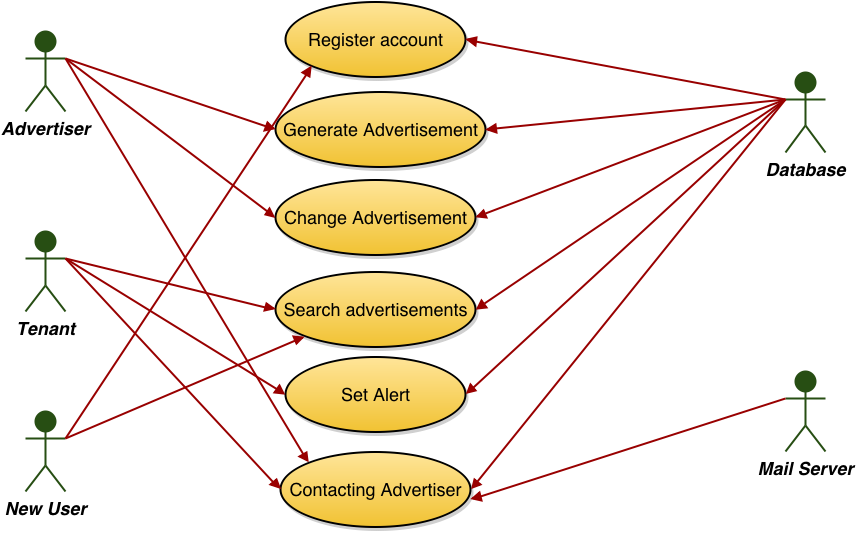
\includegraphics[width=400bp]{UseCases.png}
\end{center}

\subsection*{Login}
\begin{itemize}
	\item Actors
		\begin{itemize}
			\item User
		\end{itemize}
	\item Description
		\begin{itemize}
			\item Users have to have an account and have to be logged in in order to use advanced features like bookmarking, setting alerts and creating ads
		\end{itemize}
	\item Trigger
		\begin{itemize}
			\item User clicks the "login button"
			\item User is not logged in and clicks on one of the advanced features
			\begin{itemize}
				\item Example: User wants to bookmark an ad after a search
			\end{itemize}
		\end{itemize}
	\item Pre-Condition
		\begin{itemize}
			\item User is not logged in
		\end{itemize}
	\item Post-Condition
		\begin{itemize}
			\item User has an account
			\item User is logged in
		\end{itemize}
	\item Main Scenario
		\begin{itemize}
			\item A new user comes to studihome and would like to create an ad
			\item After clicking on the "create ad" button, he is asked to log in or to register an account
			\item If he does not have an account, he can register one (see use case "Register account")
			\item If he has an account, he can log in with his credential and is redirected to the appropriate page
		\end{itemize}
\end{itemize}

\subsection*{Register account}
\begin{itemize}
	\item Actors
		\begin{itemize}
			\item User
		\end{itemize}
	\item Description
		\begin{itemize}
			\item Every user has to have account and has to be logged in if he wants to use the more advanced features of our service.
		\end{itemize}
	\item Trigger
		\begin{itemize}
			\item Click the "register" button
		\end{itemize}
	\item Pre-Condition
		\begin{itemize}
			\item A (formally) valid email address has been entered in the form
			\item A password has been entered 
		\end{itemize}
	\item Post-Condition
		\begin{itemize}
			\item A new user has been generated
			\item The user is brought to his home screen
			\item Optional: The user receives a confirmation email
		\end{itemize}
	\item Main Scenario
		\begin{itemize}
			\item A new user comes to our web page. He does not jet have an account.
			\item He enters his email and a password of his choice
			\item A new account is created.
		\end{itemize}
\end{itemize}

\subsection*{Generate Advertisement}
\begin{itemize}
	\item Actors
		\begin{itemize}
			\item Advertiser
		\end{itemize}
	\item Description
		\begin{itemize}
			\item An advertiser wants to create an ad for his property and publish it, so interested tenants can access it.
		\end{itemize}
	\item Trigger
		\begin{itemize}
			\item The event is initialized by pressing the button "create advert"
		\end{itemize}
	\item Pre-Condition
		\begin{itemize}
			\item User is logged in
		\end{itemize}
	\item Post-Condition
		\begin{itemize}
			\item An advertisement object is created
				\begin{itemize}
					\item The minimal information requirements are
					\begin{itemize}
						\item address
						\item rent
						\item room size
						\item room number
					\end{itemize}
					\item The advertiser is free to give additional information if required
				\end{itemize}
			\item The ad is visible in "my adverts" on the advertisers page
			\item The ad is visible for other users and can be searched for
		\end{itemize}
	\item Main Scenario
		\begin{itemize}
			\item The advertiser clicks the appropriate button
			\item A UI is opened where he can enter all the information he wants
			\item He submits his ad by clicking the appropriate button
			\item He is redirected to his home
		\end{itemize}
\end{itemize}

\subsection*{Change Advertisement}
\begin{itemize}
	\item Actors
		\begin{itemize}
			\item Adertiser
		\end{itemize}
	\item Description
		\begin{itemize}
			\item Advertisements have a definite lifespan and they might change. The advertiser can therefor edit his own advertisements, close them or keep them open for longer then normal.
		\end{itemize}
	\item Trigger
		\begin{itemize}
			\item Clicking the appropriate button in the web gui
		\end{itemize}
	\item Pre-Condition
		\begin{itemize}
			\item Advertisement is open
			\item User is logged in
			\item User owns the advertisement (Has created it himself)
		\end{itemize}
	\item Post-Condition
		\begin{itemize}
			\item Changes are uploaded and the ad is saved
			\item Optional: Tenants having bookmarked this ad are informed about the change
		\end{itemize}
	\item Main Scenario
		\begin{itemize}
			\item A advertiser realizes, he has forgotten an important information in his advertisement or that it is about to be expired
			\item He logges on to his account, finds the ad in question and clicks on it
			\item The edit view is opened and he can make his modifications and prolong the ad
			\item He submits the changed form and is shown a confirmation
			\item The ad is alway in edit mode for its owner.
		\end{itemize}
\end{itemize}
\subsection*{Search advertisements}
\begin{itemize}
	\item Actors
		\begin{itemize}
			\item Tenant
			\item New User (no account)
		\end{itemize}
	\item Description
		\begin{itemize}
			\item The basic search function in which users can search for advertisements.
		\end{itemize}
	\item Trigger
		\begin{itemize}
			\item The user clicks search in the main window
			\item The user hits the enter button while the search window is active
		\end{itemize}
	\item Pre-Condition
		\begin{itemize}
			\item None
		\end{itemize}
	\item Post-Condition
		\begin{itemize}
			\item A list with all the ads matching the search criteria is shown
			\item (The list is just the list off all open ads if no keywords have been entered.
		\end{itemize}
	\item Main Scenario
		\begin{itemize}
			\item A user finds StudiHome (our web service) and uses the search field.
		\end{itemize}
\end{itemize}

\subsection*{Set Alert (Tenant)}
\begin{itemize}
	\item Actors
		\begin{itemize}
			\item Tenant
		\end{itemize}
	\item Description
		\begin{itemize}
			\item The tenant wants to be informed if a new ad matching certain user defined criteria is published.
		\end{itemize}
	\item Trigger
		\begin{itemize}
			\item An alarm is set in the search window
		\end{itemize}
	\item Pre-Condition
		\begin{itemize}
			\item One or more search keyword have been entered
			\item The user is logged in
		\end{itemize}
	\item Post-Condition
		\begin{itemize}
			\item An alarm is set
			\item The user will receive a message every time an ad matching his criteria is published
		\end{itemize}
	\item Main Scenario
		\begin{itemize}
			\item A logged in user is searching for an item but he is not happy with the result
			\item He can set his current search queue as alarm
			\item Every time a new item with these criteria is published, the user receives a message
		\end{itemize}
\end{itemize}

\subsection*{Show interest in advertisement}
\begin{itemize}
  \item Actors
    \begin{itemize}
      \item Advertiser
      \item Tenant
    \end{itemize}
  \item Description
    \begin{itemize}
      \item Tenant is interested in advertisment and wants to show it.
    \end{itemize}
 \item Trigger
    \begin{itemize}
      \item Tenant clicks “show interested" button in advertisement
    \end{itemize}
  \item Pre-conditions
    \begin{itemize}
    \item Tenant is logged in.
    \item Advertisement is open (not closed or expired)
    \item Tenant and Advertiser have valid email addresses
    \end{itemize}
  \item Post-conditions
    \begin{itemize}
      \item Interest is displayed in web app for advertiser
      \item Advertiser receives notification email
      \item Advertisement is marked as “i'm interested”
    \end{itemize}
  \item Main Scenario
    \begin{itemize}
      \item Tenants clicks “show interest” button
      \item Advertiser receives notification
    \end{itemize}
\end{itemize}

\subsection*{Contact advertiser}
\begin{itemize}
  \item Actors
    \begin{itemize}
      \item Advertiser
      \item Tenant
    \end{itemize}
  \item Description
    \begin{itemize}
      \item Tenant is interested in advertisment and wants to contact advertiser.
    \end{itemize}
 \item Trigger
    \begin{itemize}
      \item Tenant clicks “contact" button in advertisement
    \end{itemize}
  \item Pre-conditions
    \begin{itemize}
    \item Tenant is logged in.
    \item Advertisement is open (not closed or expired)
    \item Tenant and Advertiser have valid email addresses
    \end{itemize}
  \item Post-conditions
    \begin{itemize}
      \item Interest is displayed in web app for advertiser
      \item Advertiser receives notification email
    \end{itemize}
  \item Main Scenario
    \begin{itemize}
      \item Tenants clicks “contact” button
      \item Advertiser receives notification
    \end{itemize}
\end{itemize}

\subsection*{Advertiser invites tenant for visit}
\begin{itemize}
  \item Actors
    \begin{itemize}
      \item Tenant
      \item Advertiser
    \end{itemize}
  \item Description
    \begin{itemize}
      \item Advertiser wants to arrange visits with tenants who are interested in his advertisement
    \end{itemize}
  \item Trigger
    \begin{itemize}
      \item Tenant clicks the "show interest" button (See other case)
    \end{itemize}
  \item Pre-Condition
    \begin{itemize}
      \item Advertisement is open
      \item Notification email was received 
    \end{itemize}
  \item Post-Condition
    \begin{itemize}
      \item Tenant receives invitation email
      \item If the tenant agrees to the date, an event for both parties is generated
    \end{itemize}
  \item Main Scenario
    \begin{itemize}
      \item Advertiser receives notification email
      \item Advertiser logs on and sees, who's interested in his advertisement
      \item Advertiser select message ...
      \item ... and select time slots for visite
      \item Click “send”
      \item Notification email is send to tenant 
    \end{itemize}
  \end{itemize}

\subsection*{Advertiser writes message to tenant}
\begin{itemize}
  \item Actors
    \begin{itemize}
      \item Advertiser
      \item Tenant
    \end{itemize}
  \item Description
    \begin{itemize}
      \item Advertiser wants to send a message to an interested tenant
    \end{itemize}
  \item Trigger
    \begin{itemize}
      \item Advertiser receives notification (See other use case)
    \end{itemize}
  \item Pre-Condition
    \begin{itemize}
      \item Advertisement is open
      \item Notification email was received
    \end{itemize}
  \item Post-conditions
    \begin{itemize}
      \item Tenant receives notification mail
      \item Tenant receives message (in web app)
      \item message is marked as “responded to” (Advertiser)
    \end{itemize}
  \item Main Scenario
    \begin{itemize}
      \item Advertiser receives notification email
      \item Advertiser logs on to web app and sees, who's interested in his advertisment
      \item Select message
      \item Writes new message
      \item Click “send”
      \item Email is send to tenant 
      \item Message is marked as “responded to”
    \end{itemize}
\end{itemize}

%\subsection*{Tenant is no longer interested in ad}
%\begin{itemize}
%	\item Actors
%		\begin{itemize}
%			\item Tenant
%		\end{itemize}
%	\item Description
%		\begin{itemize}
%			\item A tenant changes his opinion and an ad he bookmarked or even declared a serious interest in (contacted the advertiser) is no longer seen as desirable. He therefore wants to remove the ad from his bookmarks
%		\end{itemize}
%	\item Trigger
%		\begin{itemize}
%			\item Clicking the appropriate button
%		\end{itemize}
%	\item Pre-Condition
%		\begin{itemize}
%			\item Ad is bookmarked
%			\item Ad is open
%			\item User is logged in
%		\end{itemize}
%	\item Post-Condition
%		\begin{itemize}
%			\item Ad is no longer listed under bookmarked ads
%			\item If the tenant has contacted the advertiser, the second is notified about the change
%		\end{itemize}
%	\item Main Scenario
%		\begin{itemize}
%			\item A tenant has received more information about a bookmarked ad and decides that he is no longer interested in it.
%			\item He selects the ad.
%			\item He clicks the button that removed
%	\end{itemize}
%\end{itemize}


%\subsection*{Usecase - Template}
%\begin{itemize}
%	\item Actors
%		\begin{itemize}
%			\item
%		\end{itemize}
%	\item Description
%		\begin{itemize}
%			\item
%		\end{itemize}
%	\item Trigger
%		\begin{itemize}
%			\item
%		\end{itemize}
%	\item Pre-Condition
%		\begin{itemize}
%			\item
%		\end{itemize}
%	\item Post-Condition
%		\begin{itemize}
%			\item
%		\end{itemize}
%	\item Main Scenario
%		\begin{itemize}
%			\item
%		\end{itemize}
%\end{itemize}


\end{document}
